SymPy includes several submodules that allow users to solve domain specific
physics problems. For example, a comprehensive physics submodule is included
that is useful for solving problems in mechanics, optics, and quantum
mechanics along with support for manipulating physical quantities with units.


\subsection{Classical Mechanics}
One of the core domains that SymPy suports is the physics of classical
mechanics. This is in turn separated into two distinct components:
vector algebra and mechanics.

\subsubsection{Vector Algebra}
% TODO This section requires some citations.

The \verb|sympy.physics.vector| submodule provides reference frame-, time-,
and space-aware vector and dyadic objects that allow for three-dimensional
operations such as addition, subtraction, scalar multiplication, inner and
outer products, and cross products. The vector and dyadic objects both can be
written in very compact notation that make it easy to express the vectors and
dyadics in terms of multiple reference frames with arbitrarily defined
relative orientations. The vectors are used to specify the positions,
velocities, and accelerations of points; orientations, angular velocities, and
angular accelerations of reference frames; and forces and torques. The dyadics
are essentially reference frame-aware $3 \times 3$
tensors~\cite{tai1997generalized}. The vector and dyadic objects can be used
for any one-, two-, or three-dimensional vector algebra, and they provide a
strong framework for building physics and engineering tools.

The following Python code demonstrates how a vector is created using
the orthogonal unit vectors of three reference frames that are oriented with
respect to each other, and the result of expressing the vector in the $A$
frame. The $B$ frame is oriented with respect to the $A$ frame using Z-X-Z
Euler Angles of magnitude $\pi$, $\frac{\pi}{2}$, and
$\frac{\pi}{3}$, respectively, whereas the $C$ frame is oriented
with respect to the $B$ frame through a simple rotation about the $B$ frame's
$X$ unit vector through $\frac{\pi}{2}$.

\begin{verbatim}
>>> from sympy.physics.vector import ReferenceFrame
>>> A, B, C = symbols('A B C', cls=ReferenceFrame)
>>> B.orient(A, 'body', (pi, pi/3, pi/4), 'zxz')
>>> C.orient(B, 'axis', (pi/2, B.x))
>>> v = 1*A.x + 2*B.z + 3*C.y
>>> v
A.x + 2*B.z + 3*C.y
>>> v.express(A)
A.x + 5*sqrt(3)/2*A.y + 5/2*A.z
\end{verbatim}

\subsubsection{Mechanics}

The \verb|sympy.physics.mechanics| submodule utilizes the \texttt{sympy.\allowbreak{}physics.\allowbreak{}vector} submodule
to populate time-aware particle and rigid-body objects to fully describe the
kinematics and kinetics of a rigid multi-body system. These objects store all
of the information needed to derive the ordinary differential or differential
algebraic equations that govern the motion of the system, i.e., the equations
of motion. These equations of motion abide by Newton's laws of motion and can
handle arbitrary kinematic constraints or complex loads. The submodule
offers two automated methods for formulating the equations of motion based on
Lagrangian Dynamics~\cite{Lagrange1811} and Kane's Method~\cite{kane1985dynamics}.
Lastly, there are automated linearization routines for constrained dynamical
systems~\cite{Peterson2014}.

\subsection{Quantum Mechanics}
\label{sec:quantum}

The \verb|sympy.physics.quantum| submodule has extensive capabilities to
solve problems in quantum mechanics, using Python objects to represent the
different mathematical objects relevant in quantum theory~\cite{sakurai2011modern}:
states (bras and kets), operators (unitary, Hermitian, etc.), and basis sets, as
well as operations on these objects such as representations, tensor products,
inner products, outer products, commutators, and anticommutators. The base
objects are designed in the most general way possible to enable any particular
quantum system to be implemented by subclassing the base operators and defining
the relevant class methods to provide system-specific logic.

Symbolic quantum operators and states may be defined, and one can perform
a full range of operations with them.
\begin{verbatim}
>>> from sympy.physics.quantum import Commutator, Dagger, Operator
>>> from sympy.physics.quantum import Ket, qapply
>>> A, B, C, D = symbols('A B C D', cls=Operator)
>>> a = Ket('a')
>>> comm = Commutator(A, B)
>>> comm
[A,B]
>>> qapply(Dagger(comm*a)).doit()
-<a|*(Dagger(A)*Dagger(B) - Dagger(B)*Dagger(A))
\end{verbatim}
Commutators can be expanded using common commutator identities:
\begin{verbatim}
>>> Commutator(C+B, A*D).expand(commutator=True)
-[A,B]*D - [A,C]*D + A*[B,D] + A*[C,D]
\end{verbatim}

On top of this set of base objects, a number of specific quantum systems have
been implemented in a fully symbolic framework. These include:

\begin{itemize}

\item Many of the exactly solvable quantum systems, including simple harmonic
oscillator states and raising/lowering operators, infinite square well states,
and 3D position and momentum operators and states.

\item Second quantized formalism of non-relativistic many-body quantum
mechanics~\cite{fetter2003quantum}.

\item Quantum angular momentum~\cite{zare1988angular}. Spin operators and their
eigenstates can be represented in any basis and for any quantum numbers.
A rotation operator representing the Wigner D-matrix, which may be defined
symbolically or numerically, is also implemented to rotate spin eigenstates.
Functionality for coupling and uncoupling of arbitrary spin eigenstates is
provided, including symbolic representations of Clebsch-Gordon coefficients and
Wigner symbols.

\item Quantum information and computing~\cite{nielsen2010quantum}. Multidimensional
qubit states, and a full set of one- and two-qubit gates are provided and can
be represented symbolically or as matrices/vectors. With these building blocks,
it is possible to implement a number of basic quantum algorithms including the
quantum Fourier transform, quantum error correction, quantum teleportation,
Grover's algorithm, dense coding, etc. In addition, any quantum circuit may be
plotted using the \verb|circuit_plot| function (Figure~\ref{fig-circuitplot-qft}).


\end{itemize}

Here are a few short examples of the quantum information and computing capabilities
in \verb|sympy.physics.quantum|. Start with a simple four-qubit state and flip the second
qubit from the right using a Pauli-X gate:

\begin{verbatim}
>>> from sympy.physics.quantum.qubit import Qubit
>>> from sympy.physics.quantum.gate import XGate
>>> q = Qubit('0101')
>>> q
|0101>
>>> X = XGate(1)
>>> qapply(X*q)
|0111>
\end{verbatim}
Qubit states can also be used in adjoint operations, tensor products, inner/outer
products:
\begin{verbatim}
>>> Dagger(q)
<0101|
>>> ip = Dagger(q)*q
>>> ip
<0101|0101>
>>> ip.doit()
1
\end{verbatim}
Quantum gates (unitary operators) can be applied to transform these states and
then classical measurements can be performed on the results:
\begin{verbatim}
>>> from sympy.physics.quantum.qubit import measure_all
>>> from sympy.physics.quantum.gate import H, X, Y, Z
>>> c = H(0)*H(1)*Qubit('00')
>>> c
H(0)*H(1)*|00>
>>> q = qapply(c)
>>> measure_all(q)
[(|00>, 1/4), (|01>, 1/4), (|10>, 1/4), (|11>, 1/4)]
\end{verbatim}
\begin{figure}[htbp]
\begin{center}
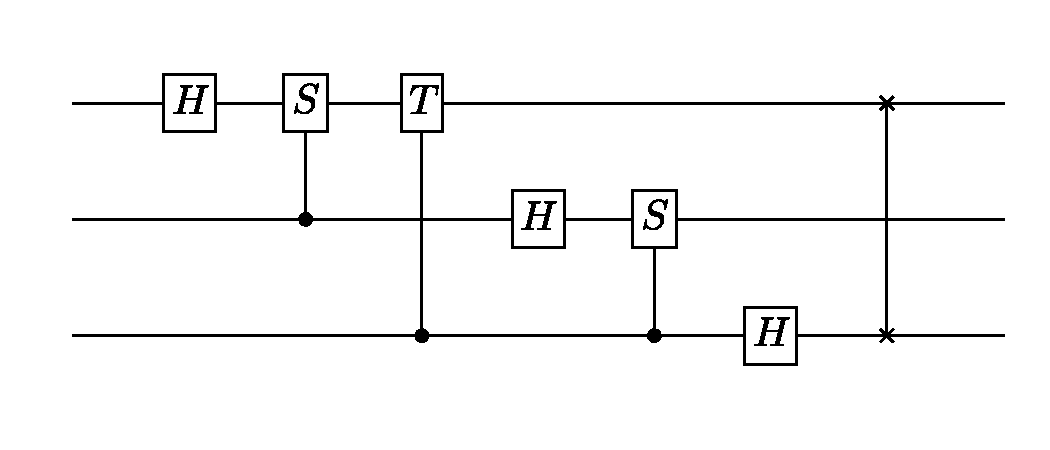
\includegraphics[scale=0.65]{images/fig1-circuitplot-qft}
\caption{The circuit diagram for a three-qubit quantum Fourier transform
generated by SymPy.}
\label{fig-circuitplot-qft}
\end{center}
\end{figure}
Lastly, the following example demonstrates creating a three-qubit quantum Fourier
transform, decomposing it into one- and two-qubit gates, and then generating a
circuit plot for the sequence of gates (see Figure~\ref{fig-circuitplot-qft}).
% This depends on matplotlib. We want to make sure the rest of the paper
% doesn't depend on it, so skip.
% no-doctest
\begin{verbatim}
>>> from sympy.physics.quantum.qft import QFT
>>> from sympy.physics.quantum.circuitplot import circuit_plot
>>> fourier = QFT(0,3).decompose()
>>> fourier
SWAP(0,2)*H(0)*C((0),S(1))*H(1)*C((0),T(2))*C((1),S(2))*H(2)
>>> c = circuit_plot(fourier, nqubits=3)
\end{verbatim}
